\documentclass[11pt, a4paper, twoside]{article}
% LTeX: language=es-AR

% Versión 1.er cuat 2021 Víctor Bettachini < vbettachini@unlam.edu.ar >

\usepackage[T1]{fontenc}
\usepackage[utf8]{inputenc}

\usepackage[spanish, es-tabla]{babel}
% \def\spanishoptions{argentina} % Was macht dass?
% \usepackage{babelbib}
% \selectbiblanguage{spanish}
% \addto\shorthandsspanish{\spanishdeactivate{~<>}}


\usepackage{graphicx}
\graphicspath{{./figuras/}{../LaTeX/}{../figurasLaTeX/}{./figs}}
% \usepackage{float}

\usepackage[arrowdel]{physics}
\newcommand{\pvec}[1]{\vec{#1}\mkern2mu\vphantom{#1}}
% \usepackage{units}
\usepackage[separate-uncertainty= true, multi-part-units= single, range-units= single, range-phrase= {~a~}, locale= FR]{siunitx}
\usepackage{isotope} % $\isotope[A][Z]{X}\to\isotope[A-4][Z-2]{Y}+\isotope[4][2]{\alpha}

\usepackage{tasks}
\usepackage[inline]{enumitem}
% \usepackage{enumerate}

\usepackage{hyperref}

% \usepackage{amsmath}
% \usepackage{amstext}
% \usepackage{amssymb}

\usepackage{tikz}
\usepackage{tikz-3dplot}
\usepackage{tikz-dimline}
\usetikzlibrary{calc}
% \usetikzlibrary{math}
\usetikzlibrary{arrows.meta}
\usetikzlibrary{snakes}
\usetikzlibrary{decorations}
\usetikzlibrary{decorations.pathmorphing}
\usetikzlibrary{patterns}

\usepackage[hmargin=1cm,vmargin=3cm, top= 0.75cm,nohead]{geometry}

\usepackage{lastpage}
\usepackage{fancyhdr}
\pagestyle{fancyplain}
\fancyhf{}
\setlength\headheight{28.7pt} 
\fancyhead[LE, LO]{\textbf{Mecánica Analítica Computacional} }
% \fancyhead[LE, LO]{\textbf{Mecánica General} }
\fancyhead[RE, RO]{\href{https://ingenieria.unlam.edu.ar/}{$\vcenter{\hbox{
\includegraphics[height=1cm]{ambos.pdf}}}$}}
\fancyfoot{\href{https://creativecommons.org/licenses/by-nc-sa/4.0/deed.es_ES}{$\vcenter{\hbox{
\includegraphics[height=0.4cm]{by-nc-sa_80x15.pdf}}}$} \href{https://ingenieria.unlam.edu.ar/}{DIIT - UNLaM}}
\fancyfoot[C]{ {\tiny Actualizado al \today} }
\fancyfoot[RO, LE]{Pág. \thepage/\pageref{LastPage}}
\renewcommand{\headrulewidth}{0pt}
\renewcommand{\footrulewidth}{0pt}

% LTeX: language = es-AR

\begin{document}
\begin{center}
  % \textsc{\large Mecánica general}\\
  \textsc{\large Ecuación de Euler-Lagrange}
\end{center}

\noindent
%De poder resolver estos problemas en forma autónoma puede asumir que adquirió los conocimientos mínimos sobre los temas abordados en la semana.
%No dude en consultar a docentes y compañeros si no puede terminarlos.
Los problemas marcados con (*) tienen alguna dificultad adicional, no dude en consultar.
\begin{enumerate} 


\item
\textbf{Péndulo rígido ideal} [Marion (english) ex. 7.2] \\
\textbf{Péndulo de punto de suspensión libre y péndulo doble} [Landau \S5 ejs. 1 y 2]\\ 
Aplique la ecuación de Euler-Lagrange para obtener las ecuaciones de la dinámica de los sistemas:
\begin{tasks}(3)
	\task 	\begin{tikzpicture}[scale= 1.3]
  	\draw [arrows=-latex] (-1,2) -> (-1,1) node [above=15, right=2] {\(\vec{g}\)}; % g vertical
		\draw [ultra thick] (-1.5,3) -- (2,3);
		\fill [pattern = north east lines] (-1.5,3) rectangle (2,3.2); % techo
		\draw [dashed] (0,3) -- (0,-.25);	% vertical
		\draw [thick] (0,3) -- +(-60:3) node[midway,above,right=2] {\(\ell\)};	% inclinada +:relativa, -60 grados, longitud 3
		\shade [ball color=black!80] ($(0,3)+(-60:3)$) circle(0.25) node [] {\color{white} $m$};
    %\draw [arrows=-latex] (0,.4) -> (1.25,.4) node [midway, above] {\( \psi \)}; % desplazamiento horizontal
		\draw [arrows=-latex] (0,0) arc [start angle=-90, end angle=-65, radius=3] node [below=12, left=8] {\( \varphi \)};
	\end{tikzpicture}
	\task 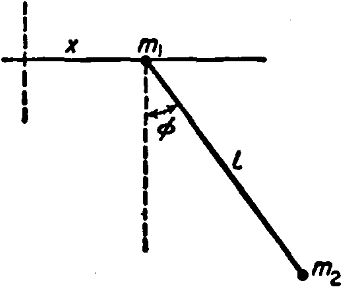
\includegraphics[height=0.23\textwidth]{landauS52_fig2}
	\task 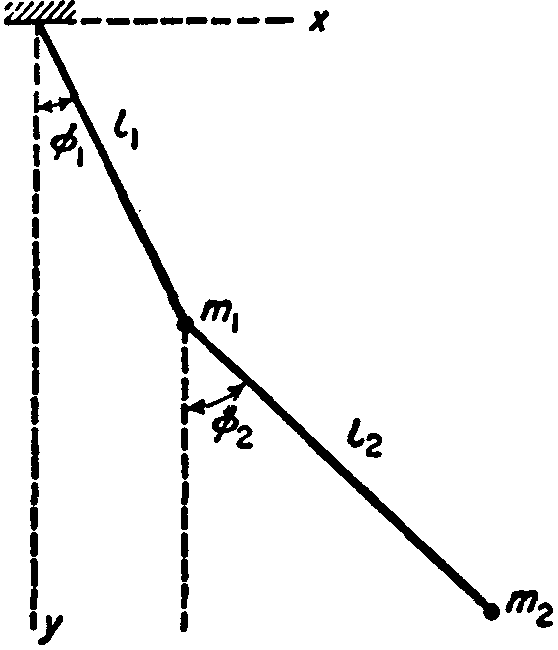
\includegraphics[height=0.23\textwidth]{landauS52_fig1}
\end{tasks}
Resultado 1c:\\
\(
\ell_{1} \left(\ell_{1} m_{1} \ddot{\varphi}_{1} + \ell_{1} m_{2} \ddot{\varphi}_{1} + \ell_{2} m_{2} \sin{\left(\varphi_{1} - \varphi_{2} \right)} \dot{\varphi}_{2}^{2} + \ell_{2} m_{2} \cos{\left(\varphi_{1} - \varphi_{2} \right)} \ddot{\varphi}_{2} + g m_{1} \sin{\left(\varphi_{1} \right)} + g m_{2} \sin{\left(\varphi_{1} \right)}\right) = 0 \\[10 pt]
\ell_{2} m_{2} \left(\ell_{1} \sin{\left(\varphi_{1} - \varphi_{2} \right)} \dot{\varphi}_{1}^{2} - \ell_{1} \cos{\left(\varphi_{1} - \varphi_{2} \right)} \ddot{\varphi}_{1} - \ell_{2} \ddot{\varphi}_{2} - g \sin{\left(\varphi_{2} \right)}\right) = 0
\)


\item
	\begin{minipage}[t][4.5cm]{0.7\textwidth}
		\textbf{Plano inclinado móvil}\\
		Un bloque de masa \(m_1\) está originalmente inmóvil sobre un plano de inclinación \(\theta\) que no le presenta fricción y de masa \(M\).
		Este último puede deslizar sobre la superficie horizontal que tampoco le presenta fricción alguna.
		Denomine con \(c\) la coordenada para la posición de este último, en la dirección y sentido indicado por la flecha; y con \(d\) la del bloque superior en el sentido descendente.
		\begin{enumerate}
			\item Obtenga la ecuación de Euler-Lagrange para \(c\) y aquella para \(d\).\\ 
			Resultado:
	\(
		M \ddot{c} - m_1 \cos{\left(\theta \right)} \ddot{d} + m_1 \ddot{c} = 0
		\qquad
		m_1 \left(g \sin{\left(\theta \right)} + \cos{\left(\theta \right)} \ddot{c} - \ddot{d }\right) = 0
	\)
				% \item (*) Intente resolver con la 2.a ley de Newton, \(\vec{F} = m \vec{a}\).
		\end{enumerate}
	\end{minipage}
	\begin{minipage}[c][0cm][t]{0.3\textwidth}
		\begin{tikzpicture}[scale= 1.3]
	% piso
	\draw [ultra thick] (-2,0) -- (1.7,0);
	\fill [pattern = north east lines] (-2,-0.2) rectangle (1.7,0);

	\draw [thick] (-1.5,0) node [above = 0.7 cm, right = 0.4 cm] {\(M\)} -- (-1.5,1.5) -- (1.5,0) -- cycle;
	\draw [arrows=-latex] (0.4,0) ++(0:0.5) arc (0:-33:-0.5) node [midway, left] {\(\theta\)};
	\draw [arrows=-Latex] (-1.6,0.7) -> (-2,0.7) node [midway, above] {\(\vec{c}\)};
	
	% Box sliding down the hypotenuse
	\coordinate (box) at (-0.5,1);
	\draw[thick,rotate around={-26:(box)}] (box) rectangle ++(1,0.5) node [midway] {\(m_1\)};
	% draw circle a a certain distance from (box)
 	\draw [arrows=-Latex, rotate={-26}] (0.3,0.9) -> (0.8,0.9) node [midway, above] {\(\vec{d}\)};
\end{tikzpicture}
		% 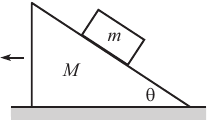
\includegraphics[width=0.75\textwidth]{cmchap6_fig6_8.png}
	\end{minipage}
	Habrá notado que no podría responder a una pregunta como ``De soltar el bloque más pequeño, ¿qué aceleración tiene el plano?'', pues obtuvo un sistema de dos ecuaciones diferenciales ligadas.
	En la clase siguiente aprenderá a resolver el sistema usando SymPy.
	



\item
	\begin{minipage}[t][4.7cm]{0.7\textwidth}
		\textbf{Soporte de péndulo sobre un plano inclinado}\\
		Un soporte de masa \(m_1\) desliza por un plano inclinado inmóvil con un ángulo \(\theta\) sin que este le presente fricción.
		Un péndulo de longitud \(\ell\) y masa \(m\) cuelga del soporte describiendo un ángulo \(\varphi\) con la vertical.
		Es soporte se extiende a un costado del plano permitiendo al péndulo colgar libremente sin interferencia de este último.
		\begin{enumerate}
			\item Encuentre las ecuaciones para la dinámica.\\
			% \item (*) Asumiendo pequeñas oscilaciones en torno a la vertical encuentre la frecuencia de oscilación del péndulo.
			Resultado:
			\(
				\ell m \left(\ell \ddot{\varphi} + g \sin{\left(\varphi \right)} + \cos{\left(\theta + \varphi \right)} \ddot{d}\right) = 0 \\[5 pt]
				\ell m \sin{\left(\theta + \varphi \right)} \dot{\varphi}^{2} - \ell m \cos{\left(\theta + \varphi \right)} \ddot{\varphi} + g m \sin{\left(\theta \right)} + g m_{1} \sin{\left(\theta \right)} - m \ddot{d} - m_{1} \ddot{d} = 0
			\)
		\end{enumerate}
	\end{minipage}
	\begin{minipage}[c][0cm][t]{0.3\textwidth}
		\begin{tikzpicture}[scale= 1.3]
	% piso
	\draw [ultra thick] (-2,0) -- (1.7,0);
	\fill [pattern = north east lines] (-2,-0.2) rectangle (1.7,0);

	% plano inclinado
	\draw [thick] (-1.5,0) -- (-1.5,1.5) -- (1.5,0) -- cycle;
	% arc for the angle theta
	\draw [arrows=-latex] (0.4,0) ++(0:0.5) arc (0:-33:-0.5) node [midway, left] {\(\theta\)};
	% \draw [arrows=-Latex] (-1.6,0.7) -> (-2,0.7) node [midway, above] {\(\vec{c}\)};
		
	% Box sliding down the hypotenuse
	\coordinate (box) at (-0.5,1);
	\draw[thick,rotate around={-26:(box)}] (box) rectangle ++(1,0.5) node [midway, below = 1 mm, right= -1 mm] {\(m_1\)};
 	\draw [arrows=-Latex, rotate={-26}] (0.3,0.9) -> (0.8,0.9) node [midway, above] {\(\vec{d}\)};

	\draw [very thick] (box) ++(0.5,0) -- ++(-0.5,-1.7) node [midway, left] {\(\ell\)};
	
	\shade [ball color=black!80] (-0.5,-0.7) circle(0.25) node [] {\color{white} $m$};

	\draw [dashed] (box) ++(0.5,0) -- ++(0,-1.95);
	% arc from the vertical previous very thick line marking angle varphi
	\draw [arrows=-latex] (box) ++(0.5,-1.4)  arc (-90:-99:2.5) node [midway, right= 2 mm] {\(\varphi\)};

\end{tikzpicture}
		% 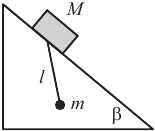
\includegraphics[width=0.75\textwidth]{cmchap6_fig6_18.png}
	\end{minipage}
	


\item
	\begin{minipage}[t][3.9cm]{0.75\textwidth}
		\textbf{Resorte enrollado en un brazo de una ``T''}\\
		Una pieza rígida en forma de T consiste en una larga varilla soldada perpendicularmente a otra de longitud \(\ell\) que pivotea en torno a un origen.
		La T gira sobre un plano horizontal con velocidad angular constante \(\omega\).
		Una partícula de masa \(m\) muy superior a la de la T, por la que esta última es despreciable, puede desplazarse libremente en la primera varilla y está conectada a la intersección de ambas por un resorte de constante elástica \(k\) y longitud natural nula.
	\end{minipage}
	\begin{minipage}[c][1cm][t]{0.3\textwidth}
		\begin{tikzpicture}
% Define coordinates
\coordinate (O) at (0,0); % Origin point

% Draw a rod at 40 degrees to the horizontal of length 2
\begin{scope}[rotate = 40]
  \draw[very thick] (O) -- (2,0) node[midway, right] {$\ell$};
  \draw[very thick] (2,2) -- (2,-2);
	\shade [ball color=black!80] (2, 1.25) circle(0.25) node [] {\color{white} $m$};
  \draw[decorate, decoration= {coil, amplitude=1.5mm, segment length=1.5 mm}] (2,0) -- (2,1) node[midway,below left] {$k$};
  % \filldraw[black] (2,1.5) circle (1.5mm) node[above right] {$m$};
\end{scope}

% Draw pivot point
\draw[black, fill=white] (O) circle (1.5 mm);
\filldraw[black] (O) circle (0.5 mm);

% arrow around 0 from angle 60 to 120
\draw[-Latex] (.5,0.5) arc (60:120:1) node[midway, above]{\(\omega\)};


\end{tikzpicture}
		% 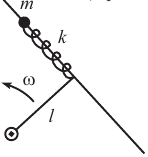
\includegraphics[width=0.75\textwidth]{cmchap6_fig6_27.png}
	\end{minipage}
	\begin{enumerate}
		\item  Encuentre una ecuación para la dinámica en función de \(d\), la distancia de la partícula a la intersección.\\
		Resultado: \(- \omega^{2} m d + k d + m \ddot{d} = 0\)
		% \item (*) Escriba \(d(t)\) asumiendo las condiciones iniciales que desee.
		%	Esto implica resolver la ecuación diferencial de segundo orden que obtuvo en el punto anterior.
		%	No utizará SymPy para resolverla, sino su conocimientos de matemática adquiridos en las asignaturas correlativas anteriores a esta.
		%	La solución debiera resultarle familiar pues no es otra que la solución para un péndulo ideal, la de un oscilador armónico simple.
		\item (*) Existe un ``valor especial'' para \(\omega\). ¿Cuál sería y que implicaría para \(d(t)\)?
		% Note que puede responder esto sin haber resuelto el punto anterior.
	\end{enumerate}


\end{enumerate}
\end{document}
